%        File: report.tex
%     Created: Fri Mar 04 10:00 AM 2016 E
% Last Change: Fri Mar 04 10:00 AM 2016 E
%
\documentclass[a4paper]{article}

\usepackage[a4paper, margin=1.25in]{geometry}

\usepackage{listings}
\usepackage{mathtools}
\usepackage{amsmath}
\usepackage{amssymb}
\usepackage{newlfont}
\usepackage{caption}
\usepackage{subcaption}
\usepackage{titlesec}
\usepackage{empheq}
\usepackage{pdfpages}
\usepackage{enumitem}
\usepackage{bm}

\newcommand{\eref}[1]{Eq.~(\ref{#1})}
\newcommand{\erefs}[2]{Eq.s~(\ref{#1}-\ref{#2})}
\newcommand{\dint}[1]{\int_{\Omega_i}{#1 d\Omega}}
\newcommand{\sint}[1]{\int_{\Gamma_{ij}}{#1 d\Gamma}}
\newcommand{\average}[1]{\ensuremath{\{#1\}} }
\newcommand{\jump}[1]{\ensuremath{[\![#1]\!]} }
\newcommand{\vbasis}{\boldsymbol{\tau}}
\newcommand{\glift}{\boldsymbol{\delta}}
\newcommand{\llift}{\boldsymbol{\delta_l}}
\newcommand{\unitn}{\mathbf{n}}
\newcommand{\mm}{\mathbf{M}}
\newcommand{\vr}{\mathbf{r}}

%\newcommand{\d}{\partial}

\title{MAE 766 Written Preliminary Exam \#1}

\author{ Kyle B. Thompson }

\begin{document}
\maketitle

\section{Introduction}
Discontinuous Galerkin (DG) methods have seen significant development in the last
three decades.  Incorporating aspects of finite-volume and finite-element
methods, DG schemes offer a compact way of achieving higher order accuracy by
solving for polynomial basis coefficients that are defined uniquely on each
element.  Discontinuities at the element boundaries are reconciled via ``flux
functions'', which provide the means that information is propagated between
elements.  This is a significant advantage when solving hyperbolic partial
differential equations (PDEs) with discontinuities in the solution, since these
discontinuities can be handled properly by flux functions using an upwind
mechanism.  Unfortunately, DG method becomes problematic when dealing with
elliptic PDEs.  Since there is not an upwinding mechanism for the diffusion
operator, a central difference seems to be an intuitive choice; however, this
has been shown to result in an inconsistent scheme. The central difference flux
does not capture jumps in the solution, only in the solution gradients.  To
overcome this issue, Bassi and Rebay developed a flux scheme\cite{br2} to account for
jumps in the solution via ``local lifting operators'', which ``lift'' the
solution to account for $C_0$ continuity.

\section{Problem Definition and Method of Solution}

Potential theory states that for incompressible flows that are irrotational, the
velocity potential function of a flow is governed by the Laplace Equation
\begin{equation}
  \Delta \phi = 0
  \label{laplace-equation}
\end{equation}
In two space dimensions this can be written out explicitly as
\begin{equation}
  \frac{\partial^2 \phi}{\partial x^2} 
  + \frac{\partial^2 \phi}{\partial y^2} = 0
  \label{2d-laplace}
\end{equation}
and the velocity is equivalent to the gradient of the potential function
\begin{equation}
  u = \frac{\partial \phi}{\partial x}, \qquad v = \frac{\partial \phi}{\partial y}
  \label{uv-def}
\end{equation}
The second scheme derived by Bassi and Rebay (BR2) solves this problem by
rewriting \eref{laplace-equation} as a first order system to be solved 
\begin{align}
  \nabla \cdot q &= 0 \\
  q - \nabla \phi &= 0
  \label{first-order-sys}
\end{align}
with $q$ being a vector auxiliary variable with dimensionality of the problem.
We proceed by defining the solution $\phi$ as a polynomial \begin{equation}
  \phi = \sum{\phi_i B_i}
  \label{fem-soln}
\end{equation}
where $\phi_i$ are the basis weights for the basis set $B_i$.  The solution can
now be interpolated anywhere in the computational domain, and the basis set used
here is a linear finite-element basis based on barycentric coordinates
\begin{equation}
  \begin{gathered}
    B_i = \frac{a_i x + b_i y + c_i}{D} \\
    a_i = y_j-y_k, \quad 
    b_i = -(x_j - x_k), \quad
    c_i = x_j y_k - x_k y_j  \\
    D = c_1 + c_2 + c_2
  \end{gathered}
  \label{basis}
\end{equation}
where the subscripts $_i$, $_j$, and $_k$ denote different nodes around the
triangle. This is a nodal basis, and is useful in that the exact integrals of
the basis functions are given by
\begin{align}
  \dint{B_1^{m}B_2^{n}B_3^{l}} &= D \frac{m!\ n!\ l!}{(m+n+l+2)!}
  \label{dom-integral-def} \\
  \sint{B_1^{m}B_2^{n}} &= L \frac{m!\ n!}{(m+n+1)!}
  \label{edge-integral-def}
\end{align}
Where $\Omega_i$ denotes the domain integral over the element $i$, and
$\Gamma_{ij}$ denotes the contour integral over the interface or boundary of an
element.
By introducing the ``lift operator'' concept and recasting
\eref{first-order-sys} in integral form, it is possible to arrive at the
``primal formulation'' that solves the system in a single equation as a function
of the solution basis weights and the lifting operators.  The first Bassi and
Rebay scheme (BR1) defined a ``global lifting operator'', $\glift$, as
\begin{equation}
  \dint{\glift \cdot \vbasis} + \sum_{j=1}^3\sint{\frac{1}{2} \jump{\phi}
  \vbasis \cdot \unitn} = 0
  \label{global-lift-def}
\end{equation}
where $\vbasis$ is an arbitrary basis function with the dimensionality of the
problem. However, using this global lifting operator was found to be
non-compact, and unstable for purely elliptic problems, such as the Laplace
equation. The BR2 scheme overcomes both of these issues by defining a ``local
lifting operator'', $\llift$, defined at each element interface by
\begin{equation}
  \begin{gathered}
    \dint{\llift \cdot \vbasis} + \eta\sint{\frac{1}{2} \jump{\phi} \vbasis
    \cdot \unitn} = 0 \\
    \jump{\phi} = \phi_i - \phi_j
  \end{gathered}
  \label{local-lift-def}
\end{equation}
Where $\eta$ is a stability parameter and $\jump{\cdot}$ is a jump operator.  It
has been proven that $\eta \geq N_{edges}$ results in a stable scheme.
Additionally, since $\vbasis$ is an arbitrary basis, the global lifting operator
can be related to the local lifting operators by summing the local lift
contributions
\begin{equation}
  \glift = \sum_{e=1}^{N_{faces}}{\llift^{(e)}}
  \label{local-global-relation}
\end{equation}
With this, the primal form is given by
\begin{equation}
  \dint{(\nabla \phi - \glift)\cdot \nabla B} -
  \sum_{j=1}^{N_{faces}}\sint{\average{(\nabla \phi - \llift)\cdot\unitn}B} = 0
  \label{primal-form}
\end{equation}
where $\average{\cdot}$ is an average operator.

\section{Implementation}
Since the Laplace equation is a linear problem, it is possible to construct a
global system an solve for all unknowns simultaneously.  This is reminiscent of
the continuous Galerkin (CG) method, where a stiffness matrix was formed for the left
hand side and a load vector for the right hand side.  In the Discontinuous Galerkin
formulation, however, continuity is not enforced across elements; therefore, the
number of unknowns going from CG(P1) to DG(P1) increases from the number of
points in the mesh to the number of elements times each elements' vertices.
Additionally, if the system is to be solved implicitly, each local lifting
operator $\llift$ must be solved for as well, increasing the total number of
equations to $3(N_{elem})+N_{faces}$ at a minimum for a triangular mesh.  This
drastically increases the problem size and complexity for an implicit solver,
since a sparsity pattern must be exploited to formulate an efficient linear
solver.

An alternative to solving the system implicitly is to explicitly evolve the
solution in pseudo-time to steady state.  Adding a time derivative to
\eref{primal-form} gives
\begin{equation}
  \dint{\frac{\partial \phi}{\partial t}B} +
  \dint{(\nabla \phi - \glift)\cdot \nabla B} -
  \sum_{j=1}^{N_{faces}}\sint{\average{(\nabla \phi - \llift)\cdot\unitn}B} = 0
  \label{primal-w-time}
\end{equation}
This results in a much simpler problem to solve, and the notation can be
contracted to
\begin{equation}
  \frac{\partial \phi}{\partial t} = -\mm^{-1} \vr
  \label{simple-explicit}
\end{equation}
where $\vr$ is the residual vector and $\mm$ is the block diagonal mass matrix.
If the boundaries are not time-dependent, then we recover the solution to the
Laplace equation upon convergence, since $\vr= 0$.  The mass matrix components can be
easily computed using \erefs{dom-integral-def}{edge-integral-def}, and the
system can be inverted by hand to significantly save computational time. The time
integration is done via Runge-Kutta and the time step can be computed locally or
globally based on a CFL prescribed.  Thus, this explicit DG scheme can be
evolved from an initial state to the solution of the Laplace equation by
iteratively updating each degree of freedom until the residual is less than a
prescribed tolerance, with the local lift operators $\llift$ simply computed as
an intermediate variable.

\section{Numerical Results}
The case being solved is a channel with a circular bump.  Figure
\ref{fig:boundary-conditions} shows triangulated mesh and the Neumann boundary conditions
prescribed.  Flow in and out of the channel is the freestream velocity (1,0),
and no flux is permitted through the channel walls.
\begin{figure}[h]
  \centering
  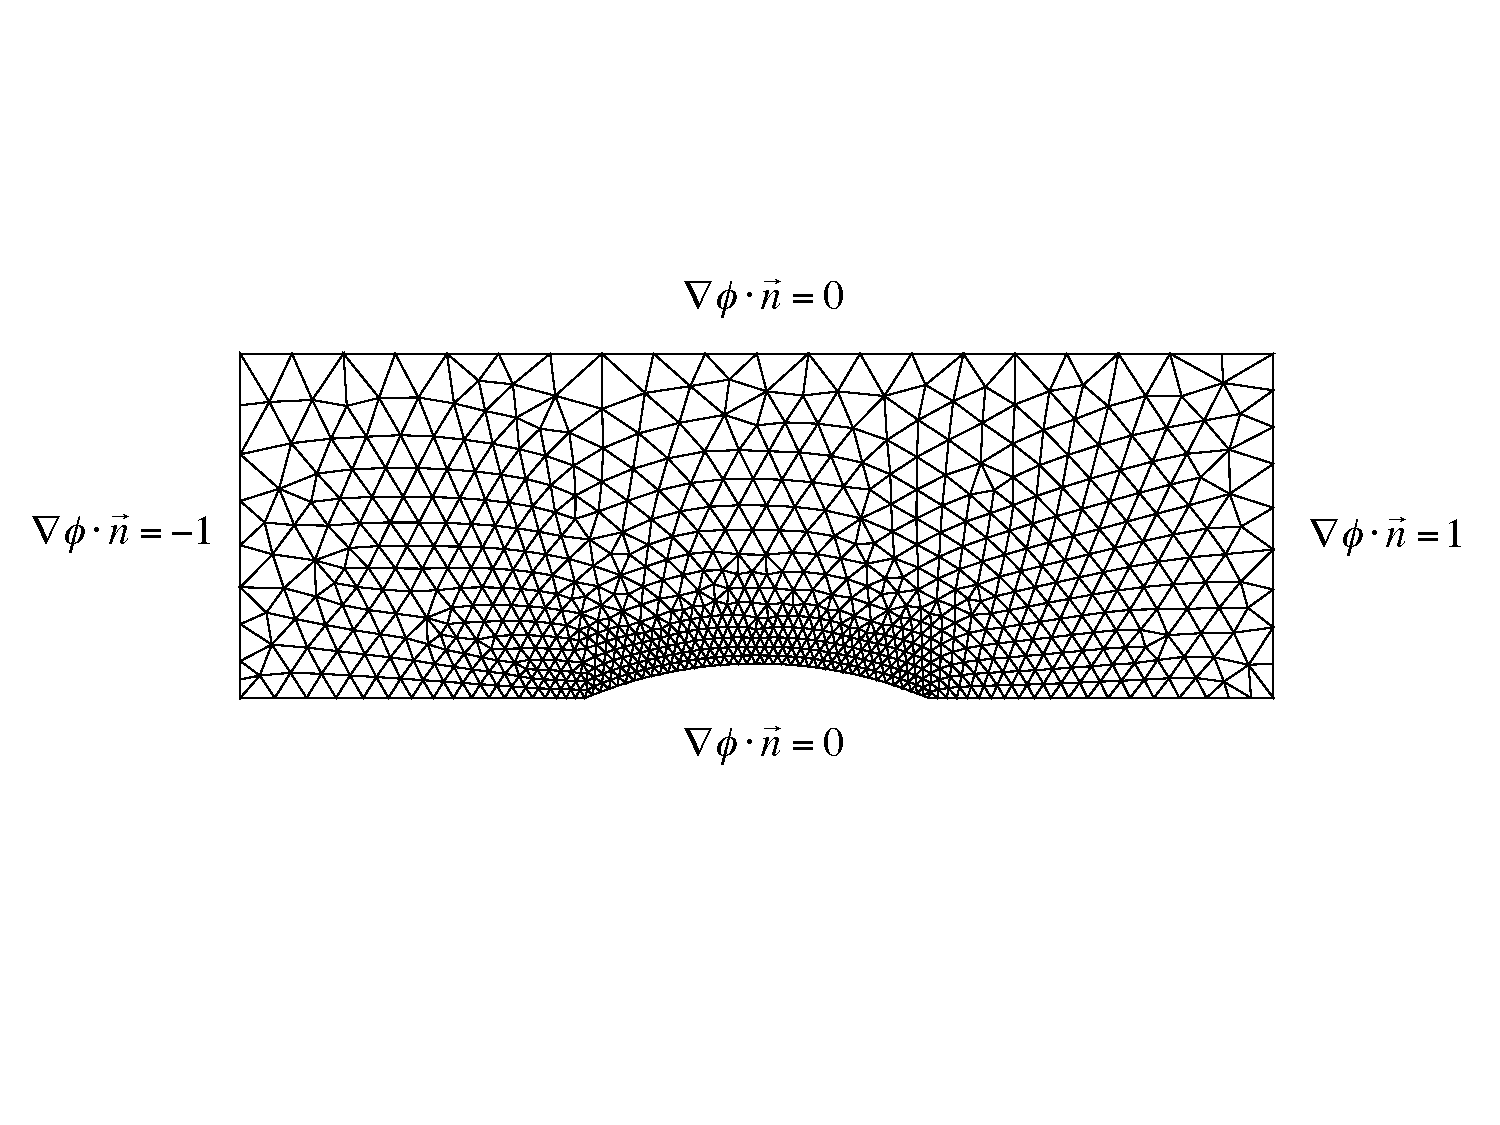
\includegraphics[width=\textwidth,trim={0 4cm 0 4cm},clip]{figures/boundary_conditions}
  \caption{Channel mesh and boundary conditions}
  \label{fig:boundary-conditions}
\end{figure}
The solution initial state was set as zero throughout the domain and evolved to
a steady state solution through explicit Runge-Kutta time integration.  The
time step used in the integration was computed locally, based on element area
and the prescribed CFL number, and the system was considered converged when the
absolute magnitude of the L2 norm of the residual was less than $10^{-12}$.
\begin{figure}[h]
  \centering
  \begin{subfigure}{0.45\textwidth}
    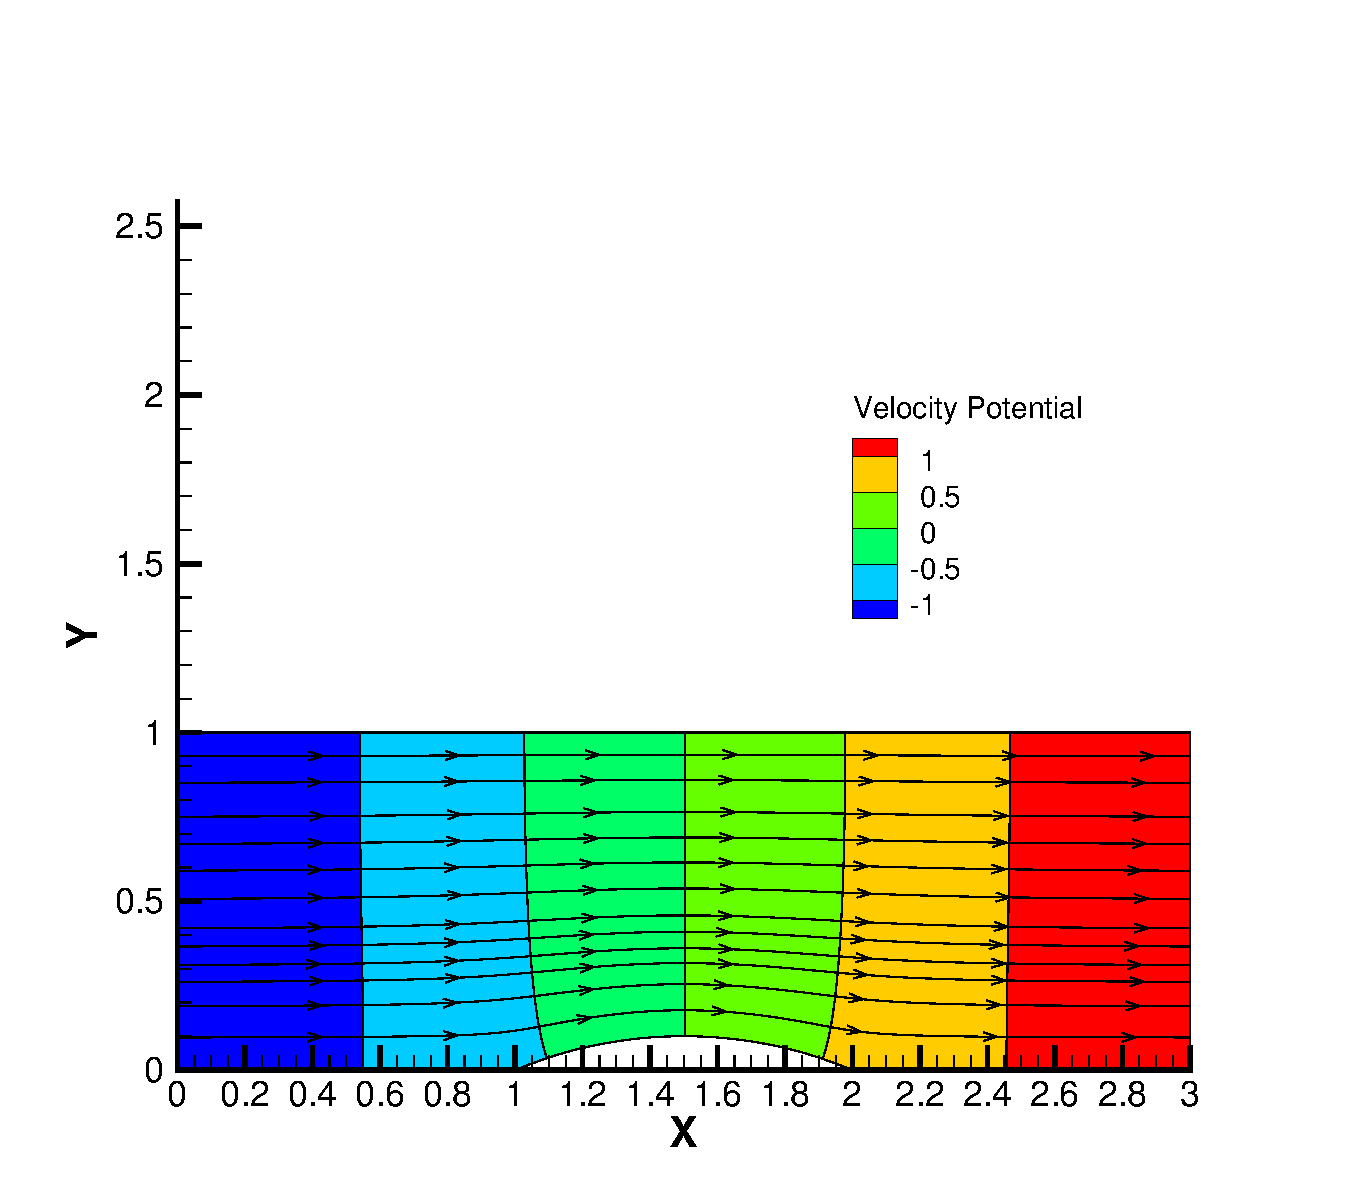
\includegraphics[width=\textwidth]{figures/potential_contour}
    \caption{Velocity potential with streamlines}
    \label{fig:potential}
  \end{subfigure}
  \begin{subfigure}{0.45\textwidth}
    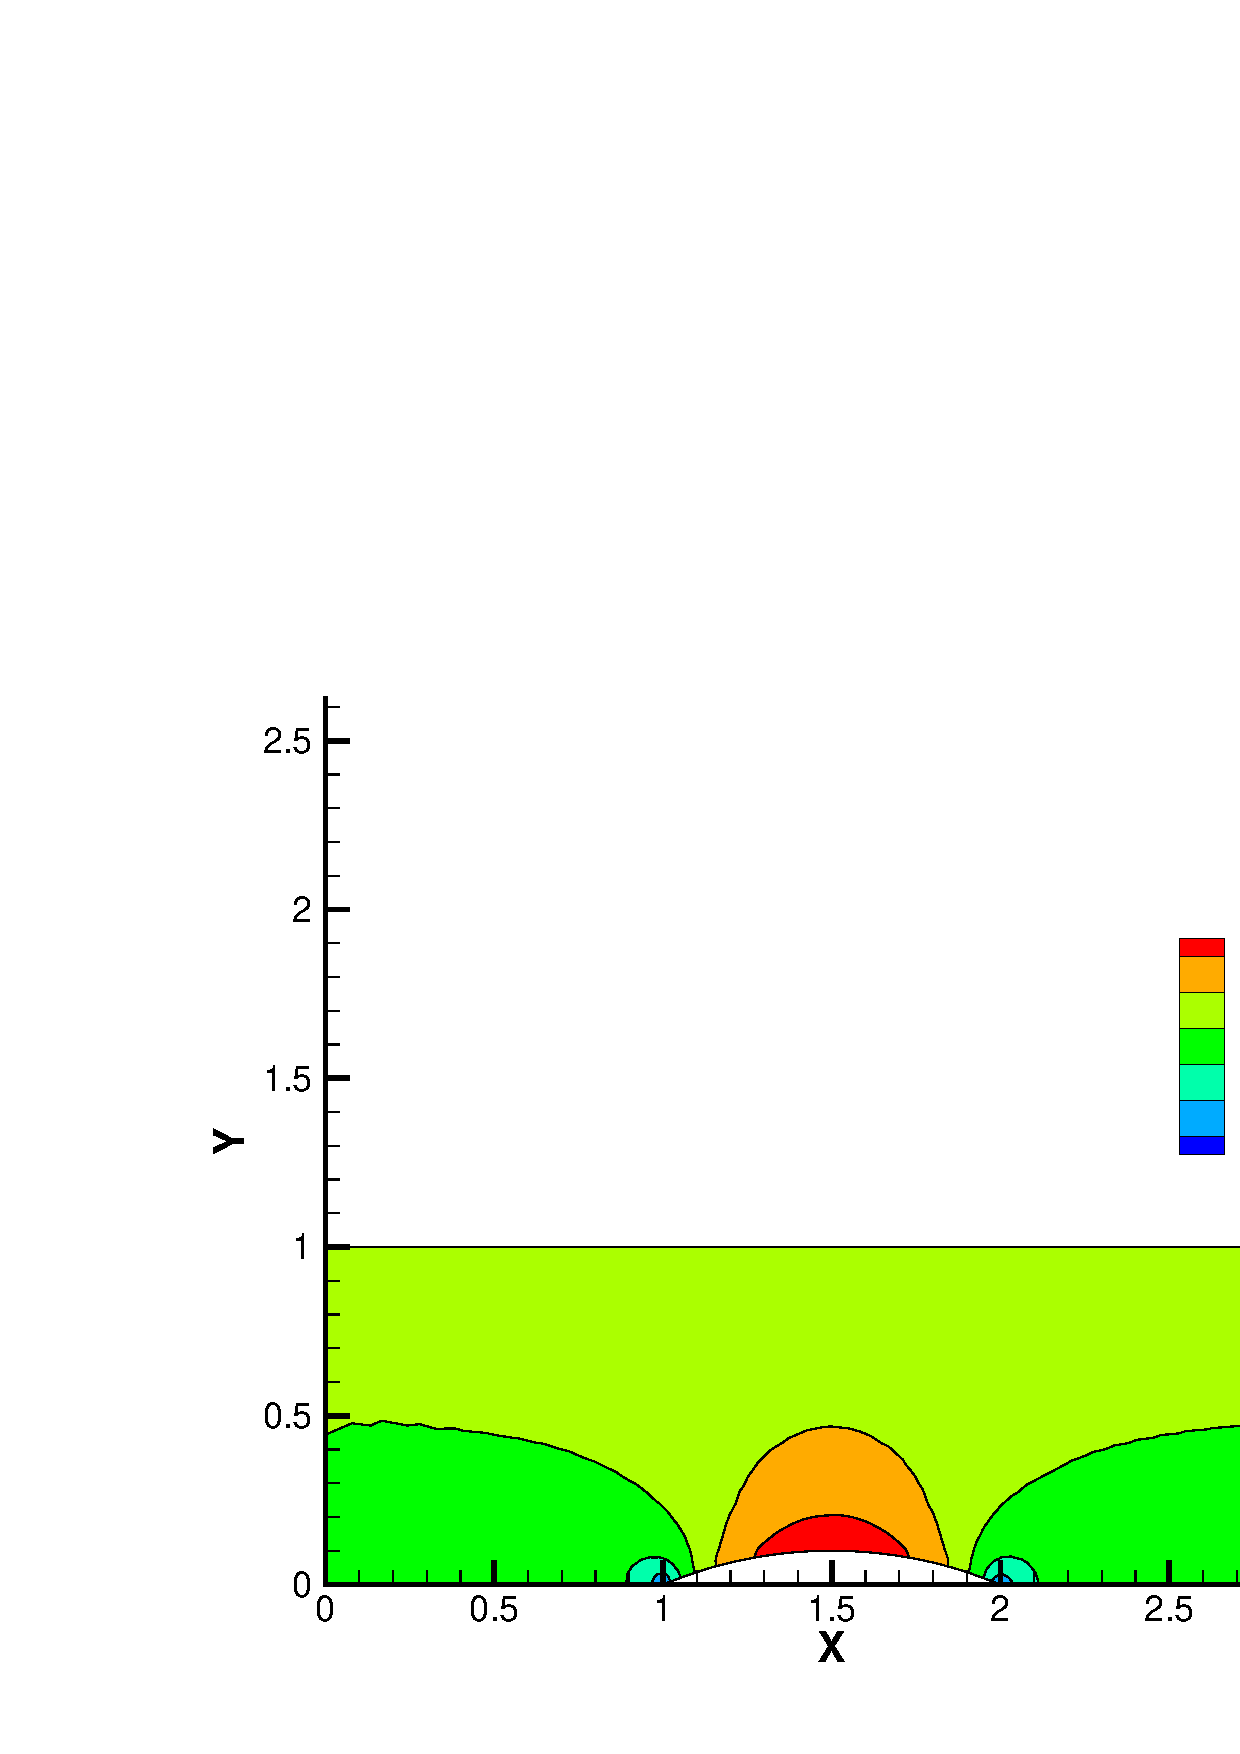
\includegraphics[width=\textwidth]{figures/Vt_contour}
    \caption{Total velocity contours}
    \label{fig:Vt-contour}
  \end{subfigure}
  \caption{Channel contour plots}
\end{figure}
Figure \ref{fig:potential} shows the velocity potential, $\phi$, contours across
the computational domain.  It is clearly seen that there is a great deal of
symmetry to this particular problem, since the geometry is mirrored across the
half-plane.  The potential behaves as expected, with the difference between the
edges of the domain and the centerline being equal in magnitude.  Figure
\ref{fig:Vt-contour} also supports the prevalence of symmetry, and shows that
the flow does indeed accelerate as it passes over the spherical bump, as
expected by the venturi effect.    
\begin{figure}[h]
  \centering
  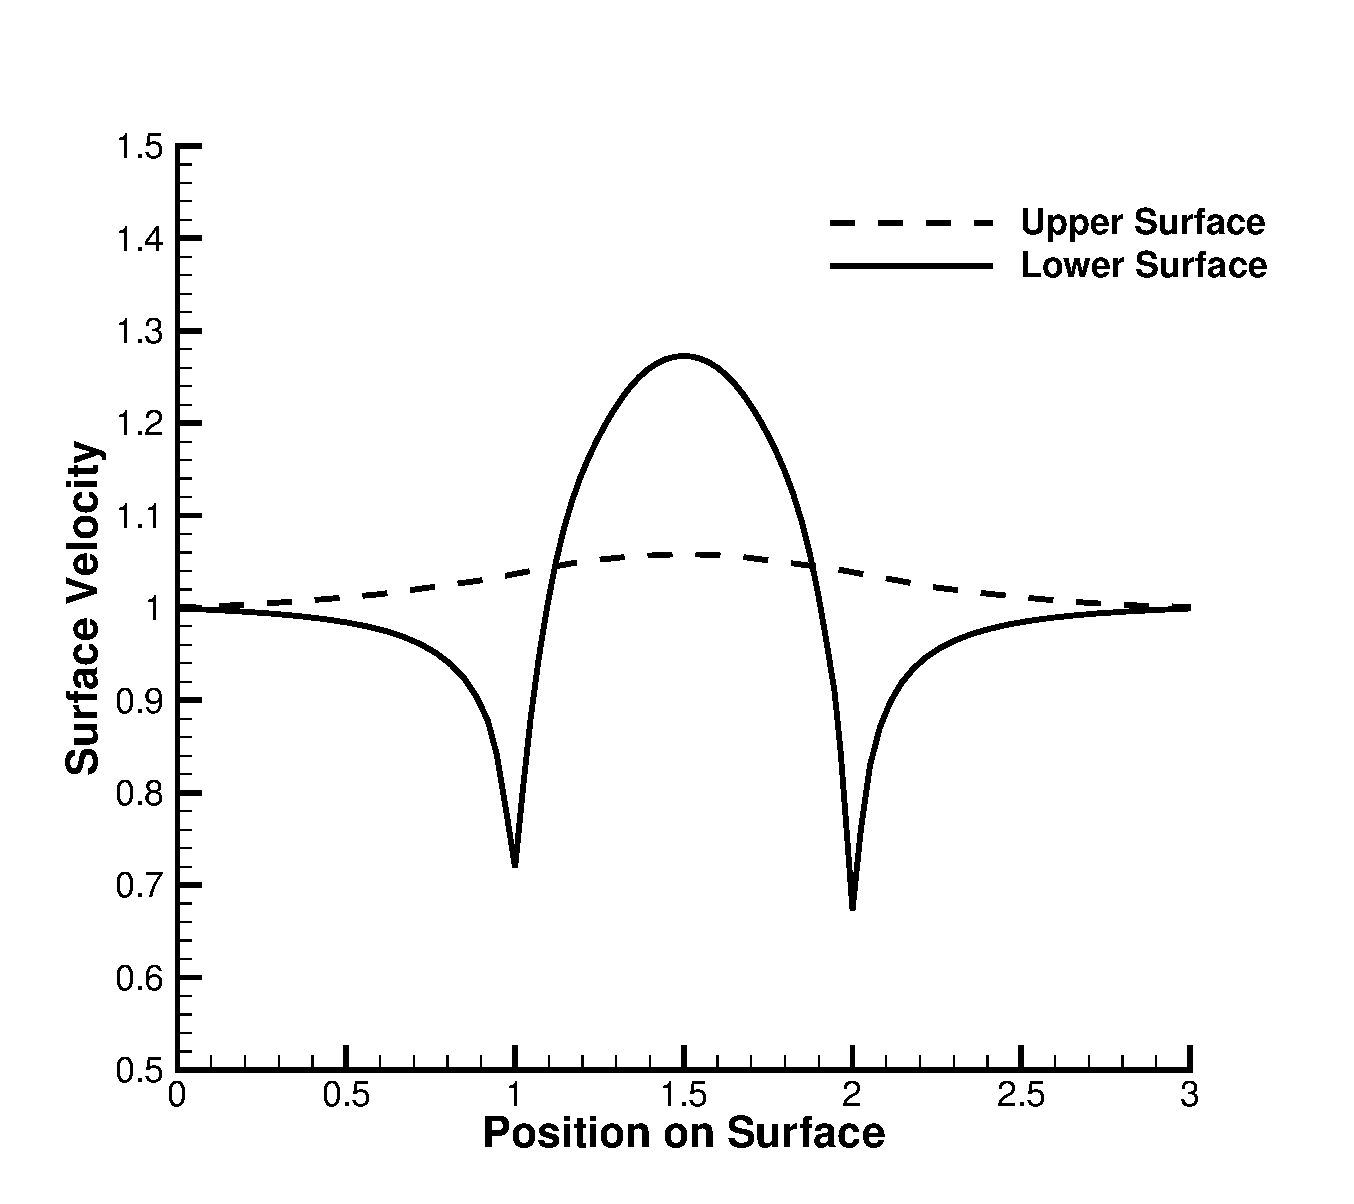
\includegraphics[width=0.5\textwidth]{figures/surface_velocity}
  \caption{Channel upper and lower surface velocity}
  \label{fig:surface-velocity}
\end{figure}
Figure \ref{fig:surface-velocity} breaks the
symmetry seen in the contour plots, as the velocity and start and end on the
bump are of equal magnitude.  Since this is potential flow over a supposedly
symmetric problem, this is unexpected, but also seen and documented by the
CG(P1) solver. Upon examining the mesh over the lower surface, it is seen that
the domain is not perfectly symmetric, and figure \ref{fig:lower-surface} shows
the point coordinates for highest point on the spherical bump are slightly off
of the half-plane. This could explain the lack of symmetry in the surface
velocity.  Another possibility is that the area-weighted averaging done to map
the solution degrees of freedom to the mesh nodes has introduced error.  A grid
refinement study and use of another averaging technique would help to better
determine what is causing the asymmetry.
\begin{figure}[h]
  \centering
  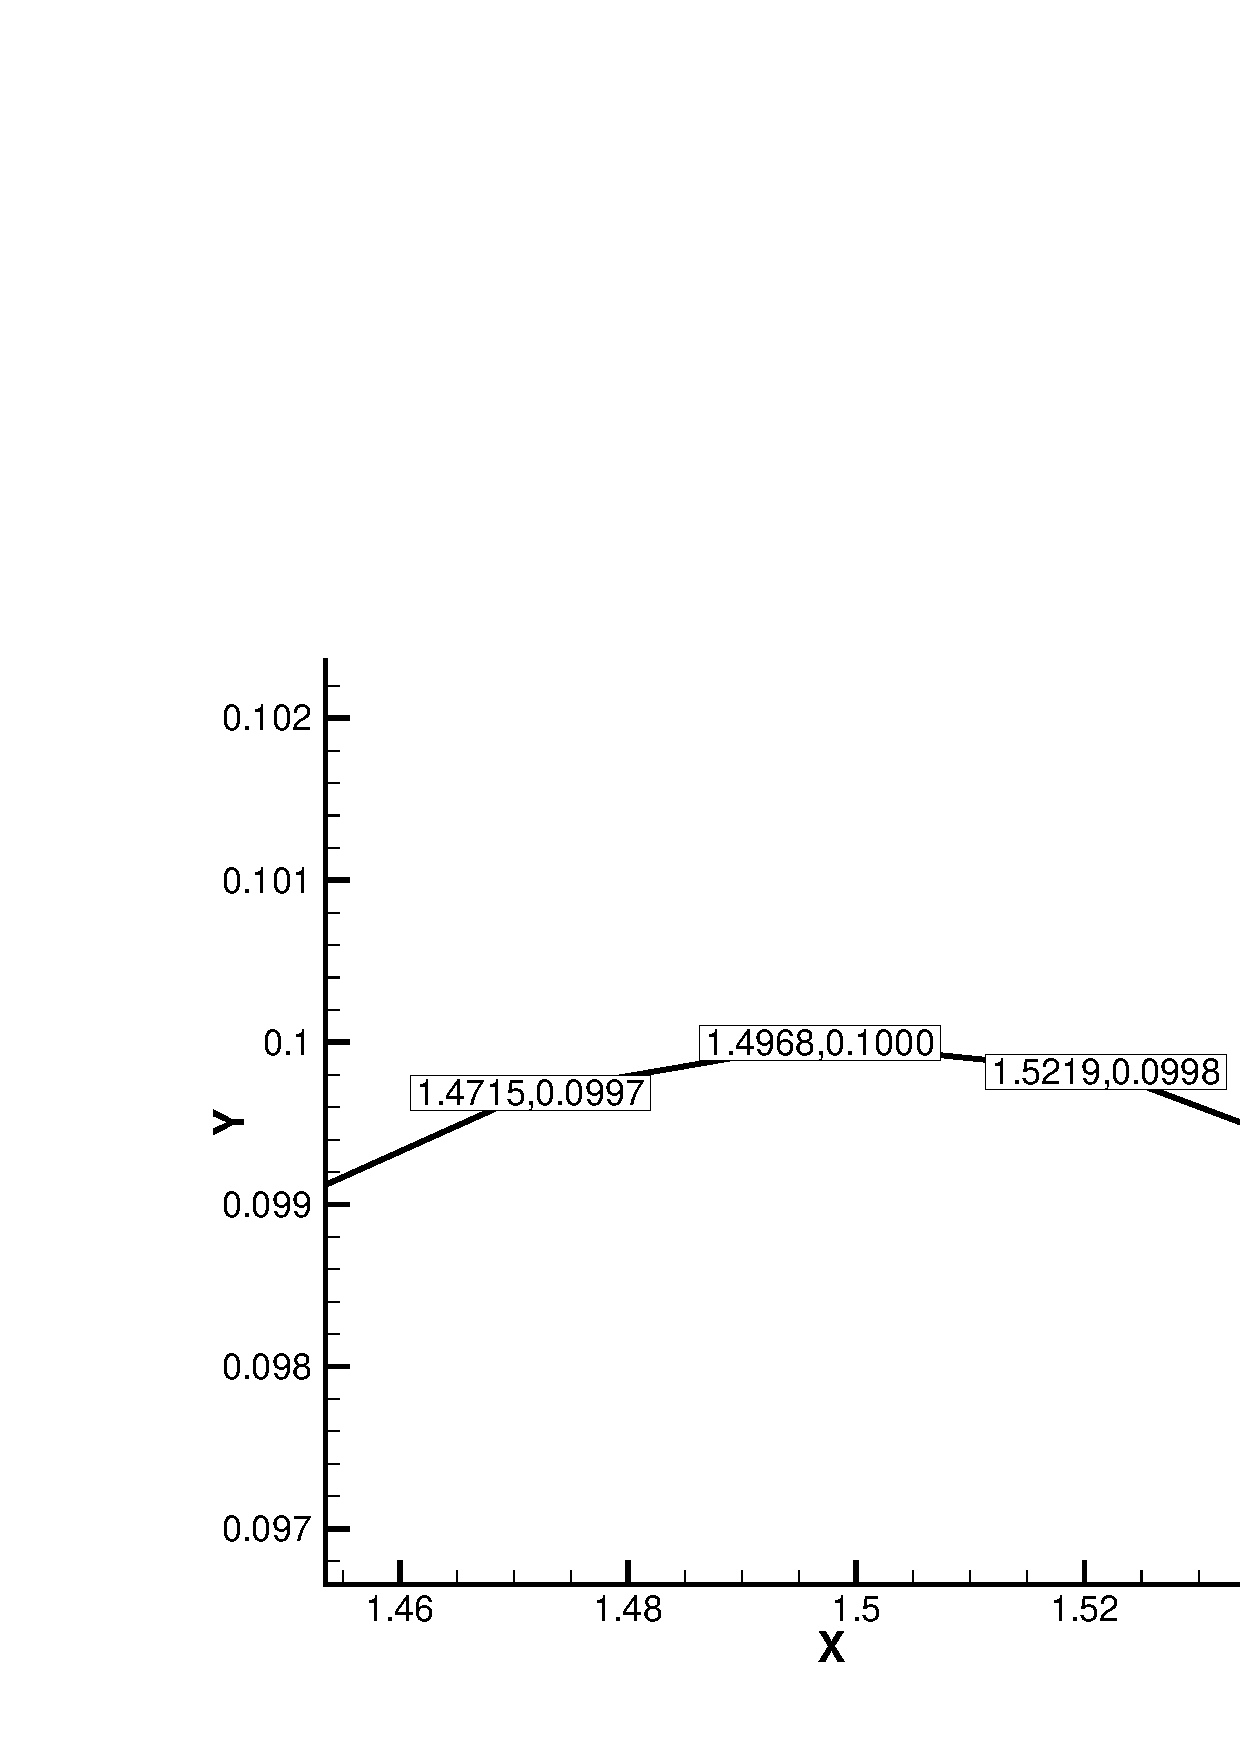
\includegraphics[width=0.5\textwidth]{figures/lower_surface}
  \caption{Channel lower surface point coordinates}
  \label{fig:lower-surface}
\end{figure}

\section{Conclusion}
The BR2 scheme provides a compact scheme that addresses the inconsistency and
stability issues associated with using DG method to solve elliptic problems.  By
integrating explicitly in pseudo-time the solution was evolved to a steady state
that satisfies the Laplace equation and gives a solution that is $C_1$ and $C_0$
continuous.  The results from the channel with a spherical bump verify that the
method is able to give results consistent with expectations, with the exception
of the minor asymmetry in the surface velocity, which may require further
analysis.

\bibliography{mae766-refs}
\bibliographystyle{plain}

\end{document}
